\chapter{Maximum Likelihood in Unsupervised Learning}
\section{Unsupervised Learning}

Recall from the beginning of our course that unsupervised learning, sometimes known as knowledge discovery, is characterised by the setting in which we have feature vectors but no labels. Formally, a dataset $\{x^{(i)}\}_{i=1}^n$ where $x^{(i)}\in\mathbb{R}^{d}$. Given such a dataset, our outlook must change from attempting to capture the unknown underlying functional relationship between inputs and outputs. Instead, the overall objective is less well-defined as attempting to understand some aspect of our data:
\begin{itemize}
    \item Is it described well by a distribution with a single mode?
    \item Is the data skewed?
    \item Are there multiple distinct but unidentified subgroups in our data?
    \item Can we approximately sample new points from our data distribution?
\end{itemize}

As we discussed in Lecture/Chapter 1, these questions are answered in tremendous detail by the many sub-areas of unsupervised learning; however, in this lecture we will focus specifically on three primary applications:
\begin{itemize}
    \item Density estimation
    \item Dimensionality reduction
    \item Briefly on data generation
\end{itemize}

\section{Density Estimation}

Consider the general unsupervised learning case where:

\[
    \mathcal{D}:=\{X_i\}_{i=1}^n
\]

where each $X_{i}$ is an i.i.d. random variable from some unknown distribution which we would like to estimate the density (PDF) of. We begin by considering these samples as single real-valued variables. Recall that an exponential family of distributions is any distribution that we can write down as:

\[
    p(\mathbf{x}=\boldsymbol{x}^{(i)}|\theta)=\frac{h(\boldsymbol{x}^{(i)})\exp(\theta^\top s(\boldsymbol{x}^{(i)}))}{z(\theta)}
\]

In the unsupervised regime, given an arbitrary setting for $\theta$ we can write the likelihood as:

\[
    p(\mathcal{D}|\theta)=\prod_{i=1}^N\frac{h(\boldsymbol{x}^{(i)})\exp(\theta^\top s(\boldsymbol{x}^{(i)}))}{z(\theta)}
\]

Which we can simplify to

\[
    p(\mathcal{D}|\theta) = z(\theta)^{-n}\exp\left(\theta^\top\sum_{i=1}^Ns(\boldsymbol{x}^{(i)}) + \sum_{i=1}^n\log h(\boldsymbol{x}^{(i)})\right)
\]
%%%%%%%%%%%%%%%%%%%%%%%%%%%%%%%%%%%%%%%%%%%%%%%%%%%%%%%%%%%%%%%%%%%%%%%%
Now, as in our previous MLE in the conditional MLE case, we will compute our gradient and set it equal to zero. Taking the log of our likelihood as a simplification step, we have:\footnote{Taking the log likelihood doesn't change the location of the maximum, but it does make the math easier.}
\[
    \log(p(\mathcal{D}|\theta)) = \underbrace{-n\log(z(\theta))}_{\text{Normalising Constant}} + \underbrace{\theta^\top s(\mathcal{D})}_{\text{Statistics}} + \underbrace{\sum\log\bigl(h(\boldsymbol{x}^{(i)})\bigr)}_{\text{Support Function } h}
\]



Differentiating both sides with respect to \( \theta_j \):

\[
    \frac{\partial}{\partial \theta_j} \log(p(\mathcal{D}|\theta)) = \frac{\partial}{\partial \theta_j} \left( -n\log(z(\theta)) + \theta^\top s(\mathcal{D}) + \sum\log\bigl(h(\boldsymbol{x}^{(i)})\bigr) \right )
\]

Since the third term does not depend on \( \theta \), its derivative is zero. Therefore, we have:

\[
    0 = -n \frac{\partial}{\partial \theta_j} \log(z(\theta)) + \frac{\partial}{\partial \theta_j} \left( \theta^\top s(\mathcal{D}) \right )
\]

First, differentiate the statistics term:

\[
    \theta^\top s(\mathcal{D}) = \sum_{j=1}^{k} \theta_j s(\mathcal{D})_j
\]

\[
    \frac{\partial}{\partial \theta_j} \theta^\top s(\mathcal{D}) = s(\mathcal{D})_j = \sum_{i=1}^N s_j(\boldsymbol{x}_i)
\]

Next, differentiate the normalising constant term. Recall that:

\[
    z(\theta) = \int_{\mathbb{R}^d} h(x) e^{\theta^{\top}s(x)} dx
\]


Now, we have one more term to differentiate, which is the normalising constant. It iswhich is a bit more challenging. Recall from our previous lecture on exponential families that the function $z(\theta)$ is a normalising constant that can always be written as: \footnote{The normalising constant is the integral of the the unnormalised density function, which includes the support function. This is so it can divide out the unnormalised function so its entire area sums to 1.}

\[
    z(\theta) = \int_{\mathbb{R}^d} h(x) e^{\theta^{\top}s(x)} dx
\]


To derive the gradient of \( \log(z(\theta)) \), we proceed as follows:

\begin{align*}
    \frac{\partial}{\partial \theta_j} \log(z(\theta)) &= \frac{1}{z(\theta)} \frac{\partial}{\partial \theta_j} z(\theta) \\
    &= \frac{1}{z(\theta)} \int_{\mathbb{R}^d} h(x) s_j(x) e^{\theta^\top s(x)} dx \\
    &= \int_{\mathbb{R}^d} s_j(x) \frac{h(x) e^{\theta^\top s(x)}}{z(\theta)} dx \\
    &= \int_{\mathbb{R}^d} s_j(x) p(x; \theta) dx \\
    &= \mathbb{E}_{x \sim p(x; \theta)} [s_j(x)]
\end{align*}

Thus, we have:

\[
    \frac{\partial}{\partial \theta_j} \log(z(\theta)) = \mathbb{E}[s_j(x)]
\]

Combining the differentiated terms, the gradient equation becomes:

\begin{align*}
    0 &= -n \mathbb{E}[s_j(x)] + \sum_{i=1}^N s_j(\boldsymbol{x}_i) \\
    \mathbb{E}[s_j(x)] &= \frac{1}{n} \sum_{i=1}^N s_j(\boldsymbol{x}_i)
\end{align*}

\hl{This implies that at the critical points of exponential distributions, the expected value of the sufficient statistics under the model equals the empirical average of the sufficient statistics from the data.This is true for any critical point of the distribution and will come in handy for the method of moments.  \bigskip

In other words, the sample mean of the sufficient statistics should equal the true mean of the sufficient statistics.}\marginnote[-30pt]{This relationship is fundamental in deriving the maximum likelihood estimates for parameters in exponential family distributions.}


% \hl{This means that at critical points of exponential distributions the sample mean of the sufficient statistics should equal the true mean of the sufficient statistics. This is true for any critical point of the distribution and will come in handy for the method of moments.}

%%%%%%%%%%%%%%%%%%%%%%%%%%%%%%%%%%%%%%%%%%%%%%%%%%%%%%%%%%%%%%%%%%%%%%%%

Another really useful fact that we saw during this derivation was the identity that:

\[
    \nabla_\theta \log(z(\theta)) = \mathbb{E}_x[s(\boldsymbol{x})]
\]

To see how this is useful, recall the definition of an exponential distribution in canonical form:

\[
    \begin{aligned}
        h(x)      & = \mathbf{I}(x \geq 0), \\
        s(x)      & = -x,                   \\
        \theta    & = \lambda,              \\
        a(\theta) & = -\log(-\theta).
    \end{aligned}
\]

Here, it is easy to see that:

\[
    \frac{\partial}{\partial\theta} \log(z(\theta)) = -\frac{1}{\theta}
\]

with $\theta = \lambda$ implies the gradient of our normalising function is $-\frac{1}{\lambda}$ which we also know is the mean of the sufficient statistic which is $-x$. Therefore, we can reason that the mean of this distribution with respect to $\boldsymbol{L}$ is $\frac{1}{\lambda}$ which may have been much more difficult to solve for had we not computed this nice, general identity.






\subsection{Method of Moments for Exponential Families:}
\marginnote[17.5pt]{
\intuitsb{Estimators for Moments}{One nice thing about the moments of a distribution is they have very straightforward estimators. The estimator for the $k^{\text{th}}$ moment given $n$ i.i.d. samples from $X$ is: $\frac{1}{n}\sum_{i=1}^{n}x_{i}^{k}$ and the estimator for the $k^{\text{th}}$ moment about $C$ is simply: $\frac{1}{n}\sum_{i=1}^{n}(x_{i}-c)^{k}$.}
}
\defb{Definition 10.2.1. Moments of a Distribution}{
    Given a random variable $U$ distributed according to $p(\boldsymbol{x})$, the $k^{\text{th}}$ moment of $U$ is defined as:

    \[
        \mathbb{E}[x^k]
    \]

    Moreover, the $k^{\text{th}}$ moment of $U$ about $C$ (for a constant $C$) is:

    \[
        \mathbb{E}[(x - C)^k]
    \]

}

Now, the method of moments (in simple terms and only for the first moment) can be expressed as setting the first true moment equal to the sample estimate of the first moment. This also generalisable to higher-order moments, where the \(k\)-th theoretical moment is equated to the \(k\)-th empirical moment to derive additional parameter estimates. \bigskip


We showed above using our computed identities that the expectation of the exponential distribution was $1/\lambda$. Now, assuming we have access to $n$ i.i.d. samples from a random variable that we want to fit using an exponential distribution, rather than computing the negative log likelihood and solving, we can use the method of moments. Observe that we know:

\[
    \mathbb{E}[x] = \frac{1}{\lambda}
\]

and that

\[
    \hat{\boldsymbol{x}}_{n} = \frac{1}{n}\sum_{i=1}^{n}x_{i}
\]

and we know that these must be equal so:

\begin{align*}
    \mathbb{E}[\boldsymbol{x}] = \frac{1}{\lambda} = \frac{1}{n}\sum_{i=1}^{n}\boldsymbol{x}_{i} \\
    \implies \lambda = \frac{1}{\frac{1}{n}\sum_{i=1}^{n}\boldsymbol{x}_{i}}
\end{align*}

Which immediately gives us our estimator for $\lambda$ which students can verify is actually equal to the MLE for this distribution. \bigskip

\section{Dimensionality Reduction}

Visualising high-dimensional data ($d > 3$) is challenging but crucial for understanding machine learning problems. 
\begin{marginfigure}
    \centering
    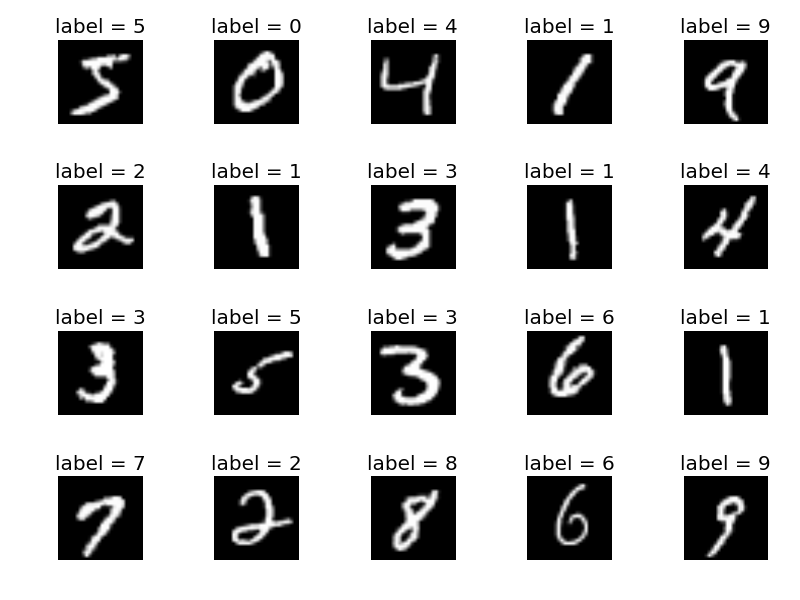
\includegraphics[width=1\linewidth]{img/2_mnist.png}
    \caption{MNIST handwritten digit dataset.}
    \label{fig:mnist_}
\end{marginfigure}
\begin{marginfigure}
    \centering
    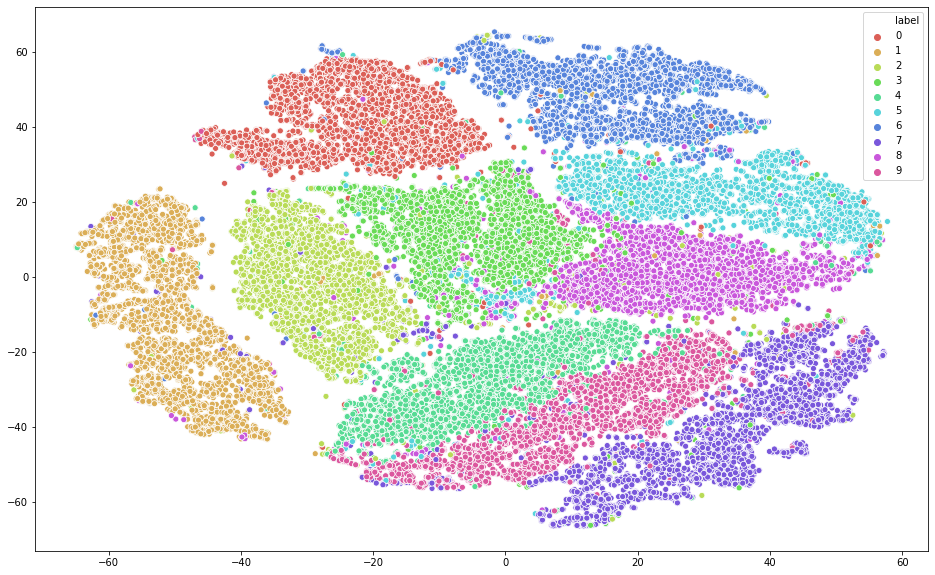
\includegraphics[width=1\linewidth]{img/2_mnist-tsne.png}
    \caption{MNIST dataset projected into 2D using t-SNE.}
    \label{fig:mnist_tsne}
\end{marginfigure}
\begin{itemize}
    \item In the MNIST handwritten digit dataset, projecting each 28$\times$28 pixel image into $\mathbb{R}^2$ allows us to estimate the number of distinct digit classes by observing the resulting point cloud.
    \item Beyond simple visualization, advanced dimensionality reduction techniques like Variational Auto-Encoders (VAEs) provide deeper insights into the underlying data structure.
    \item We will explore practical applications after introducing one of the most popular dimensionality reduction algorithms: Principal Component Analysis (PCA).
\end{itemize}

\subsection{Minimising Reconstruction Error}

To visualise data in lower dimensions, we use transformation matrices. Let $W \in \mathbb{R}^{2 \times d}$ be a matrix that projects data from $d$ to 2 dimensions. The quality of this projection is measured by the reconstruction error:
\[
    \mathcal{L}(\boldsymbol{W}) = \|\boldsymbol{x} - \boldsymbol{W}^\top(\boldsymbol{W}\boldsymbol{x})\|_2^2
\]
Here, $W^\top$ projects back from 2 to $d$ dimensions. For the entire dataset, the loss is:
\[
    \mathcal{L}(\boldsymbol{W}) = \frac{1}{n} \sum_{i=1}^n \|\boldsymbol{x}^{(i)} - \boldsymbol{W}(\boldsymbol{W}^\top \boldsymbol{x}^{(i)})\|_2^2
\]
Using the design matrix $X$ (with rows as transposed inputs), this can be rewritten as:
\[
    \mathcal{L}(\boldsymbol{W}) = \|X - X\boldsymbol{W}\boldsymbol{W}^\top\|_{\mathrm{F}}^2
\]
where $\|\cdot\|_{\mathrm{F}}^2$ denotes the squared Frobenius norm. \bigskip

To solve the optimisation problem:
\[
    \boldsymbol{W}^{\star} = \underset{W}{\operatorname{argmin}} \| \boldsymbol{X} - \boldsymbol{X}\boldsymbol{W}\boldsymbol{W}^\top \|_{\mathrm{F}}^{2}
\]
we decompose the Frobenius norm:
\[
    \|X\|_{\mathrm{F}}^{2} = \underbrace{\|X\boldsymbol{W}\boldsymbol{W}^\top\|_{\mathrm{F}}^{2}}_{\text{Aspects captured by the subspace}} + \underbrace{\|X - X\boldsymbol{W}\boldsymbol{W}^\top\|_{\mathrm{F}}^{2}}_{\text{Aspects not captured by subspace}}
\]
This implies that minimising the reconstruction error is equivalent to maximising $\|X\boldsymbol{W}\boldsymbol{W}^\top\|_{\mathrm{F}}^{2}$. However, the solution to this is not uniqe because we could arbitrarily scale $\bm{W}$ and get the same result. To ensure a unique solution, we impose that the columns of $W$ are orthonormal:
\[
    \boldsymbol{W}^\top \boldsymbol{W} = \mathbf{I}
\]

\subsection{Principal Component Analysis}

Consider our dataset as a collection of i.i.d. random variables:
\[
    \mathcal{D} = \{\mathbf{x}^{(1)}, \mathbf{x}^{(2)}, \ldots, \mathbf{x}^{(n)}\}
\]
where each $\mathbf{x}^{(i)} \in \mathbb{R}^{d}$ is a $d$-dimensional feature vector. Assume the dataset is centred, meaning the mean of each feature across all data points is zero. To summarise the shape of this centred point cloud, we use the covariance matrix $\bm{S}$:
\[
    \bm{S} = \frac{1}{n} \bm{X}^\top \bm{X}
\]
where $X \in \mathbb{R}^{n \times d}$ is the design matrix. \bigskip

The covariance matrix $\bm{S}$ captures how each feature varies with every other feature. We perform an eigen decomposition of $\bm{S}$:
\[
    \bm{S} = \bm{U} \bm{\Lambda} \bm{U}^\top
\]
where:
\begin{itemize}
    \item $\bm{U} \in \mathbb{R}^{d \times d}$ is an orthogonal matrix of eigenvectors,
    \item $\bm{\Lambda} \in \mathbb{R}^{d \times d}$ is a diagonal matrix with eigenvalues $\lambda_{1} \geq \lambda_{2} \geq \cdots \geq \lambda_{d} \geq 0$.
\end{itemize}

To reduce dimensionality while retaining maximum variance, select the top $k$ eigenvectors corresponding to the largest eigenvalues as columns of $W \in \mathbb{R}^{d \times k}$:
\[
    W = [\mathbf{u}_1, \mathbf{u}_2, \ldots, \mathbf{u}_k]
\]
These vectors are the principal components. Projecting data onto these principal components yields a $k$-dimensional representation that preserves the maximum possible variance from the original $d$ dimensions. This reduction is optimal as it minimises the reconstruction error, capturing the most significant patterns and structures in the dataset.

\subsection{Proof that Principal Components Maximise Our Objective}

To maximise $\| \bm{X}\bm{W}\bm{W}^\top \|_{\mathrm{F}}^{2}$, we expand the Frobenius norm:
\[
    \| \bm{X}\bm{W}\bm{W}^\top \|_{\mathrm{F}}^{2} = \mathrm{tr}\left( (\bm{X}\bm{W}\bm{W}^\top)^\top (\bm{X}\bm{W}\bm{W}^\top) \right)
\]
Since $(\bm{X}\bm{W}\bm{W}^\top)^\top = \bm{W}\bm{W}^\top \bm{X}^\top$, this becomes:
\[
    \mathrm{tr}(\bm{W}\bm{W}^\top \bm{X}^\top \bm{X} \bm{W}\bm{W}^\top)
\]
Using the cyclic property of trace, $\mathrm{tr}(\mathbf{AB}) = \mathrm{tr}(\mathbf{BA})$, we simplify:
\[
    \mathrm{tr}(\bm{W}\bm{W}^\top \bm{X}^\top \bm{X} \bm{W}\bm{W}^\top) = \mathrm{tr}(\bm{W}^\top \bm{X}^\top \bm{X} \bm{W})
\]
Thus, the objective reduces to:
\[
    \| \bm{X}\bm{W}\bm{W}^\top \|_{\mathrm{F}}^{2} = \mathrm{tr}(\bm{W}^\top \bm{X}^\top \bm{X} \bm{W})
\]
Performing an eigen decomposition of $\bm{X}\bm{X}^\top = \bm{U} \bm{\Lambda} \bm{U}^\top$, substitute into the expression:
\[
    \mathrm{tr}(\bm{W}^\top \bm{U} \bm{\Lambda} \bm{U}^\top \bm{W})
\]
To maximise this trace, choose $\bm{W}$ to align with the top $k$ eigenvectors of $\bm{X}\bm{X}^\top$, corresponding to the largest eigenvalues in $\bm{\Lambda}$. Therefore, setting $\bm{W}$ to be the matrix formed by the first $k$ columns of $\bm{U}$ maximises:
\[
    \mathrm{tr}(\bm{W}^\top \bm{X}^\top \bm{X} \bm{W}) = \lambda_{1} + \lambda_{2} + \cdots + \lambda_{k}
\]
This corresponds to the largest possible value of our objective $\| \bm{X}\bm{W}\bm{W}^\top \|_{\mathrm{F}}^{2}$, thereby proving that principal components maximise the captured variance.

\section{Generative Learning with Variational Auto-Encoders}

\begin{itemize}
    \item PCA can be viewed as a linear autoencoder, using a linear transformation to project data into a smaller feature space while preserving information.
    \item More complex transformations are possible, but these require advanced tools not covered in this year’s examinable material.
    \item This section serves to motivate concepts for the next lecture and provide further reading for interested students.
    \item To make PCA more expressive, a natural step is to consider basis expansion.
\end{itemize}



\subsection{Basis Expansion and Kernel PCA}

PCA is effective when the standard Euclidean norm captures meaningful relationships between points. Key considerations include:
\begin{itemize}
    \item \textbf{Objective}: Maximising captured variance is an intuitive and desirable goal.
    \item \textbf{Data Patterns}: Real-world data may exhibit complex patterns, such as radial relationships, which are not well-captured by linear projections.
    \item \textbf{Projection Function}: To address complex patterns, we can consider non-linear projections of the data, denoted as $\phi(x)$, similar to basis expansion.
    \item \textbf{Computational Challenges}: Choosing a complicated basis expansion for PCA complicates the computation of eigenvalues and eigenvectors.
    \item \textbf{Kernel Trick}: To handle complex basis expansions efficiently, the kernel trick can be employed. This technique allows us to compute the principal components in the transformed feature space without explicitly performing the transformation.
\end{itemize}

\subsection{Neural Network Autoencoders}

Another approach to dimensionality reduction involves using non-linear models instead of linear transformations. This section covers autoencoders and variational autoencoders (VAEs):
\begin{itemize}
    \item \textbf{Non-linear Models}: Eliminating linear transformations allows for capturing more complex data structures.
    \item \textbf{Autoencoders and VAEs}: These are popular models based on deep neural networks that learn efficient data representations.
    \item \textbf{Training Method}: Instead of computing principal components, these models use gradient descent to optimise their parameters.
    \item \textbf{Network Architecture}: The key idea is to introduce a bottleneck in the network with a lower dimensionality $d$:
    \begin{itemize}
        \item \textbf{Encoder}: Maps input data to a latent representation, $E(x) = z$.
        \item \textbf{Decoder}: Reconstructs the input data from the latent representation, $D(\boldsymbol{z}) = \hat{x}$.
    \end{itemize}
    \item \textbf{Objective}: By minimising the reconstruction loss, the autoencoder learns a compact representation of the data that can be used for visualization and, in some cases, to generate new data samples from the same distribution.
\end{itemize}

\subsubsection{Variational Autoencoders}

Variational Autoencoders (VAEs) address the challenge of generating new samples from the learned representation:
\begin{itemize}
    \item \textbf{Sampling Issue}: Sampling randomly from the latent representation $Z$ can be problematic if the distribution of $E(\boldsymbol{x})$ does not follow a known distribution.
    \item \textbf{Known Distribution Constraint}: To ensure meaningful generation of new samples, VAEs incorporate a loss term that penalises the difference between the output distribution of $E(\boldsymbol{x})$ and a predefined reference distribution (e.g., a normal distribution).
    \item \textbf{Regularisation}: This approach is similar to regularisation techniques previously discussed in the course, linking the penalty term to probabilistic notions.
    \item \textbf{Future Exploration}: The mathematical details of how this loss term is formulated and optimised will be covered in the next lecture.
\end{itemize}
